% !TeX root = ../main.tex

\chapter{系統設計}
自主身分(AID)系統是一種創新的身分管理方案,其核心理念在於讓每位使用者在具備\textbf{道德標準}的身分系統中\textbf{自由的管理自己},從而解決現有身分管理系統的問題。本章節將深入探討如何通過核心機制的設計將這一理念融入系統中,同時闡述系統的完整架構設計、資安與隱私議題和資料結構,為AID系統的實際應用奠定理論基礎。
\section{系統核心機制}
為了實現AID系統的核心理念,我們需要深入理解\textbf{道德標準}與\textbf{自由的管理自己}這兩個關鍵概念,並將其轉化為具體的技術機制。
\subsection{關鍵概念}
以下將分別探討道德標準和自由的管理自己這兩個關鍵概念。
\subsubsection{道德標準的建立}
就像Nietzsche所說的道德是弱者對強者的反抗,我們認為道德標準的建立並不是簡單的制定某些規範,而是創建出一種機制能讓多數普通使用者能夠集結力量,形成共識,從而有效地制衡可能濫用權力的少數強勢參與者。因此,AID系統引入了一種基於區塊鏈的去中心化評價機制。在這個機制中:
\begin{itemize}
  \item 每個系統參與者(包括使用者和服務提供商)都有權對其他參與者進行評價。
  \item 這些評價被記錄在區塊鏈上,確保其不可篡改和公開透明。
  \item 系統參與者可以按照自己的需求分析其他參與者的評價,從而形成對其道德標準的判斷。
\end{itemize}
通過這種機制,AID系統實現了一種基於共識的道德標準,使得每位使用者都能夠參與到對系統的建設和監督中,從而確保系統道德標準的建立。\newpage
\subsubsection{自由的管理自己}
為了實現使用者對自己身分的自主管理,我們需要深入了解自主身分系統中可管理的元素。在AID系統架構中,使用者可管理的內容包括兩個方面:
\begin{enumerate}
  \item \textbf{數據管理}:指使用者在系統交互過程中產生的全部數據。
  \item \textbf{功能管理}:指只能由使用者自己決定要行使哪些功能。
\end{enumerate}
\begin{figure}
  \centering
  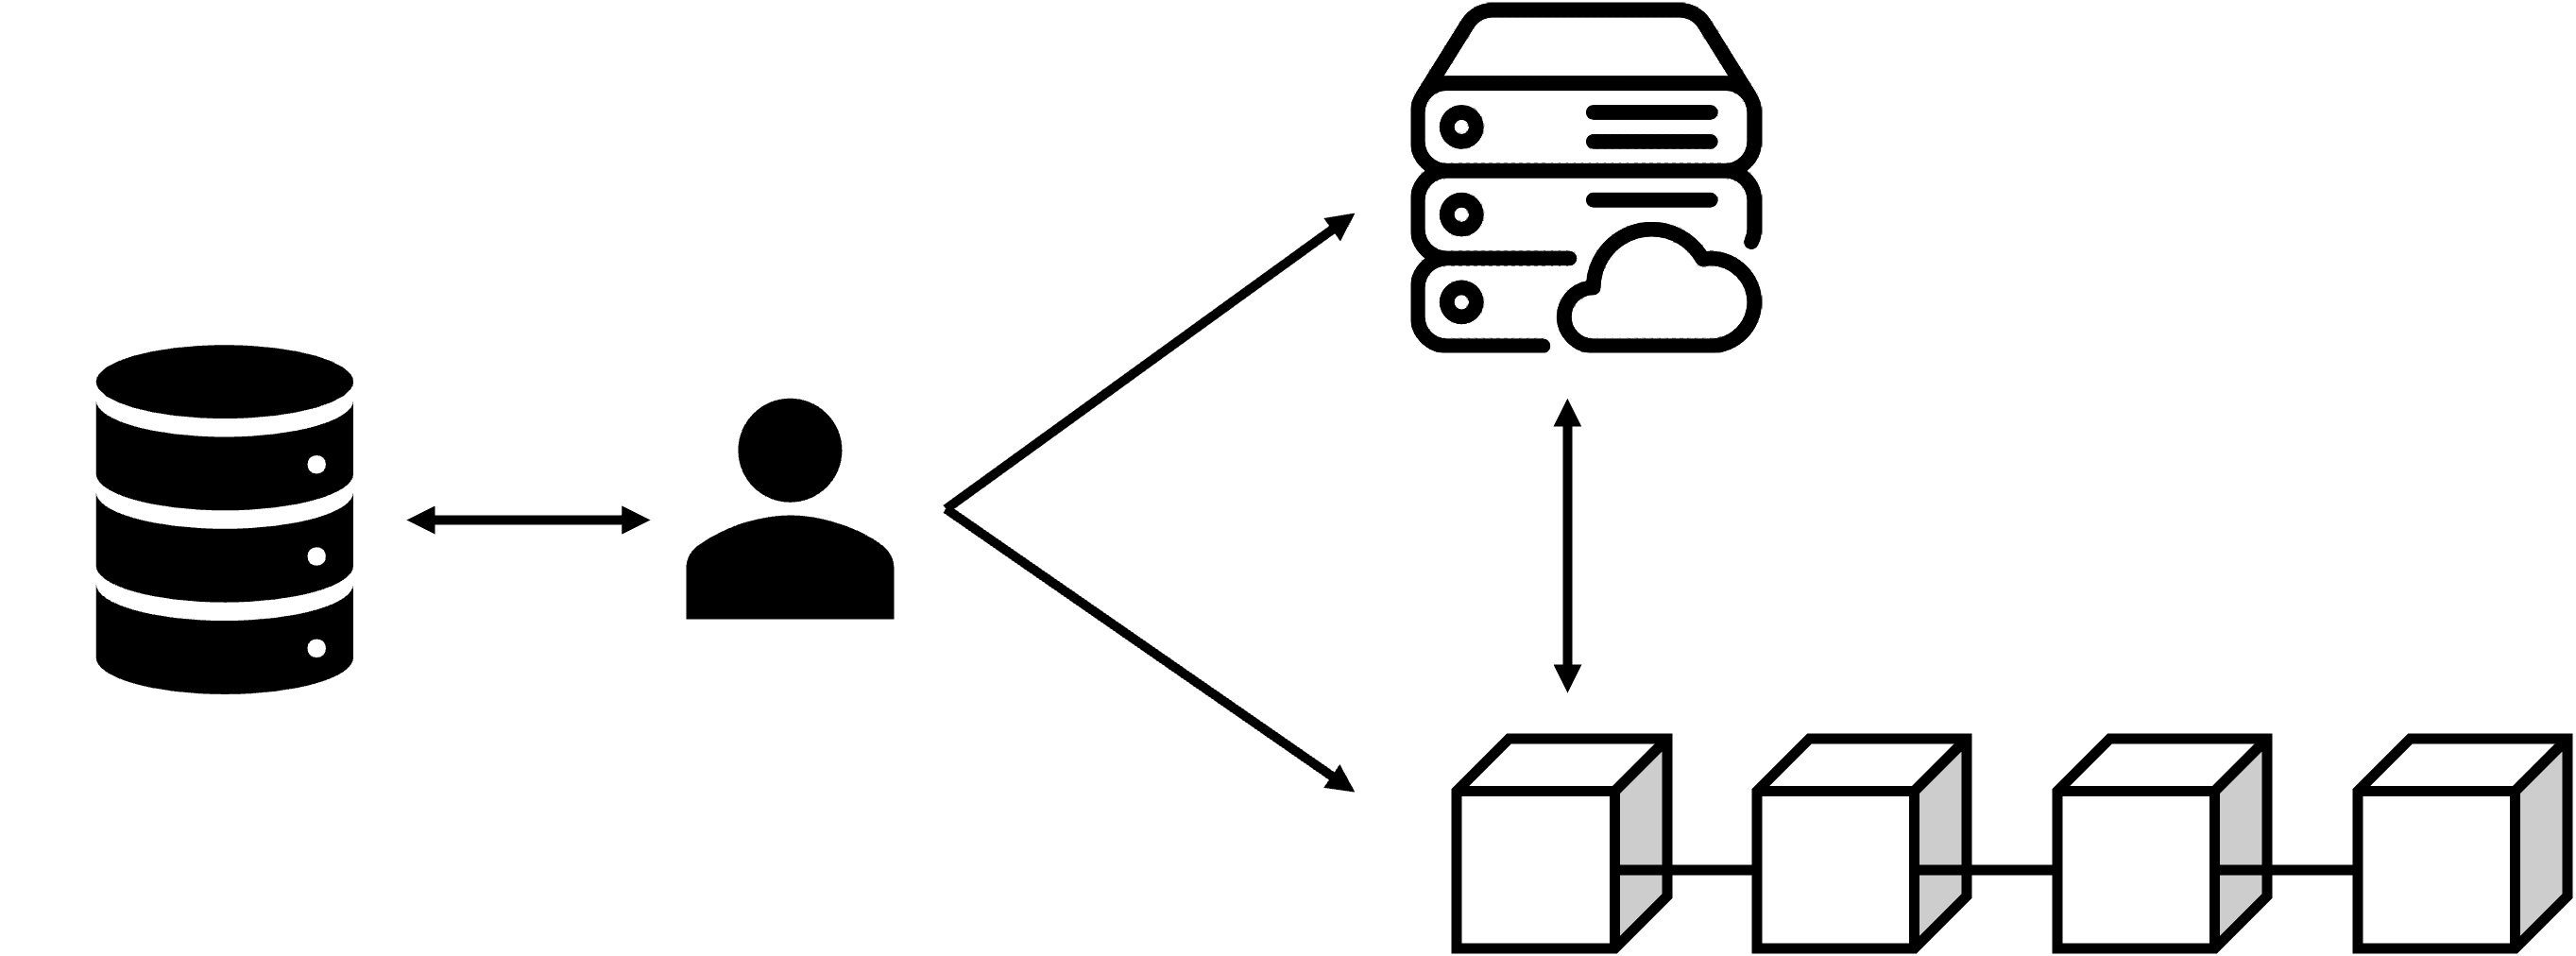
\includegraphics[width=\linewidth,keepaspectratio]{figures/aid.png}
  \caption{自主身分}
  \label{fig:aid}
\end{figure}
實現數據的自由管理是一項具有挑戰性的任務。在傳統身分管理系統中,使用者數據通常由身分供應商(Identity Provider)或服務提供商(Service Provider)集中控制,這嚴重限制了使用者在個人數據上的自由。為了克服這一限制,AID系統採用了創新的「數據層反轉」策略如圖\ref{fig:aid}:將使用者數據完全遷移至使用者端設備,從而實現使用者對個人數據的直接控制。

與此同時,在功能管理方面,AID系統摒棄了管理者或任何形式的中心化控制方法。這樣的設計進一步增強了使用者管理自身身分的自由度,再次彰顯了自主身分的核心理念。
\subsection{技術機制}
基於上述關鍵概念,我們要強調幾項與之相關的重要技術機制。
\subsubsection{自主證照}
為了實現使用者能夠自由加入服務而無需在服務中存儲個人數據,同時允許其他系統參與者對使用者進行評價,我們參考了Tze-Nan\cite{NTU202102846}提出的自主證照概念,設計了一個基於區塊鏈技術的自主身分管理流程。

自主證照是由使用者自行生成的一種證照,使用者可以根據個人需求自定義證照的內容和權限,並且擁有隨時撤銷證照的權力。這種機制讓使用者能夠靈活地管理自己的身分信息,同時確保了系統的安全性和可靠性。
\begin{figure}
  \centering
  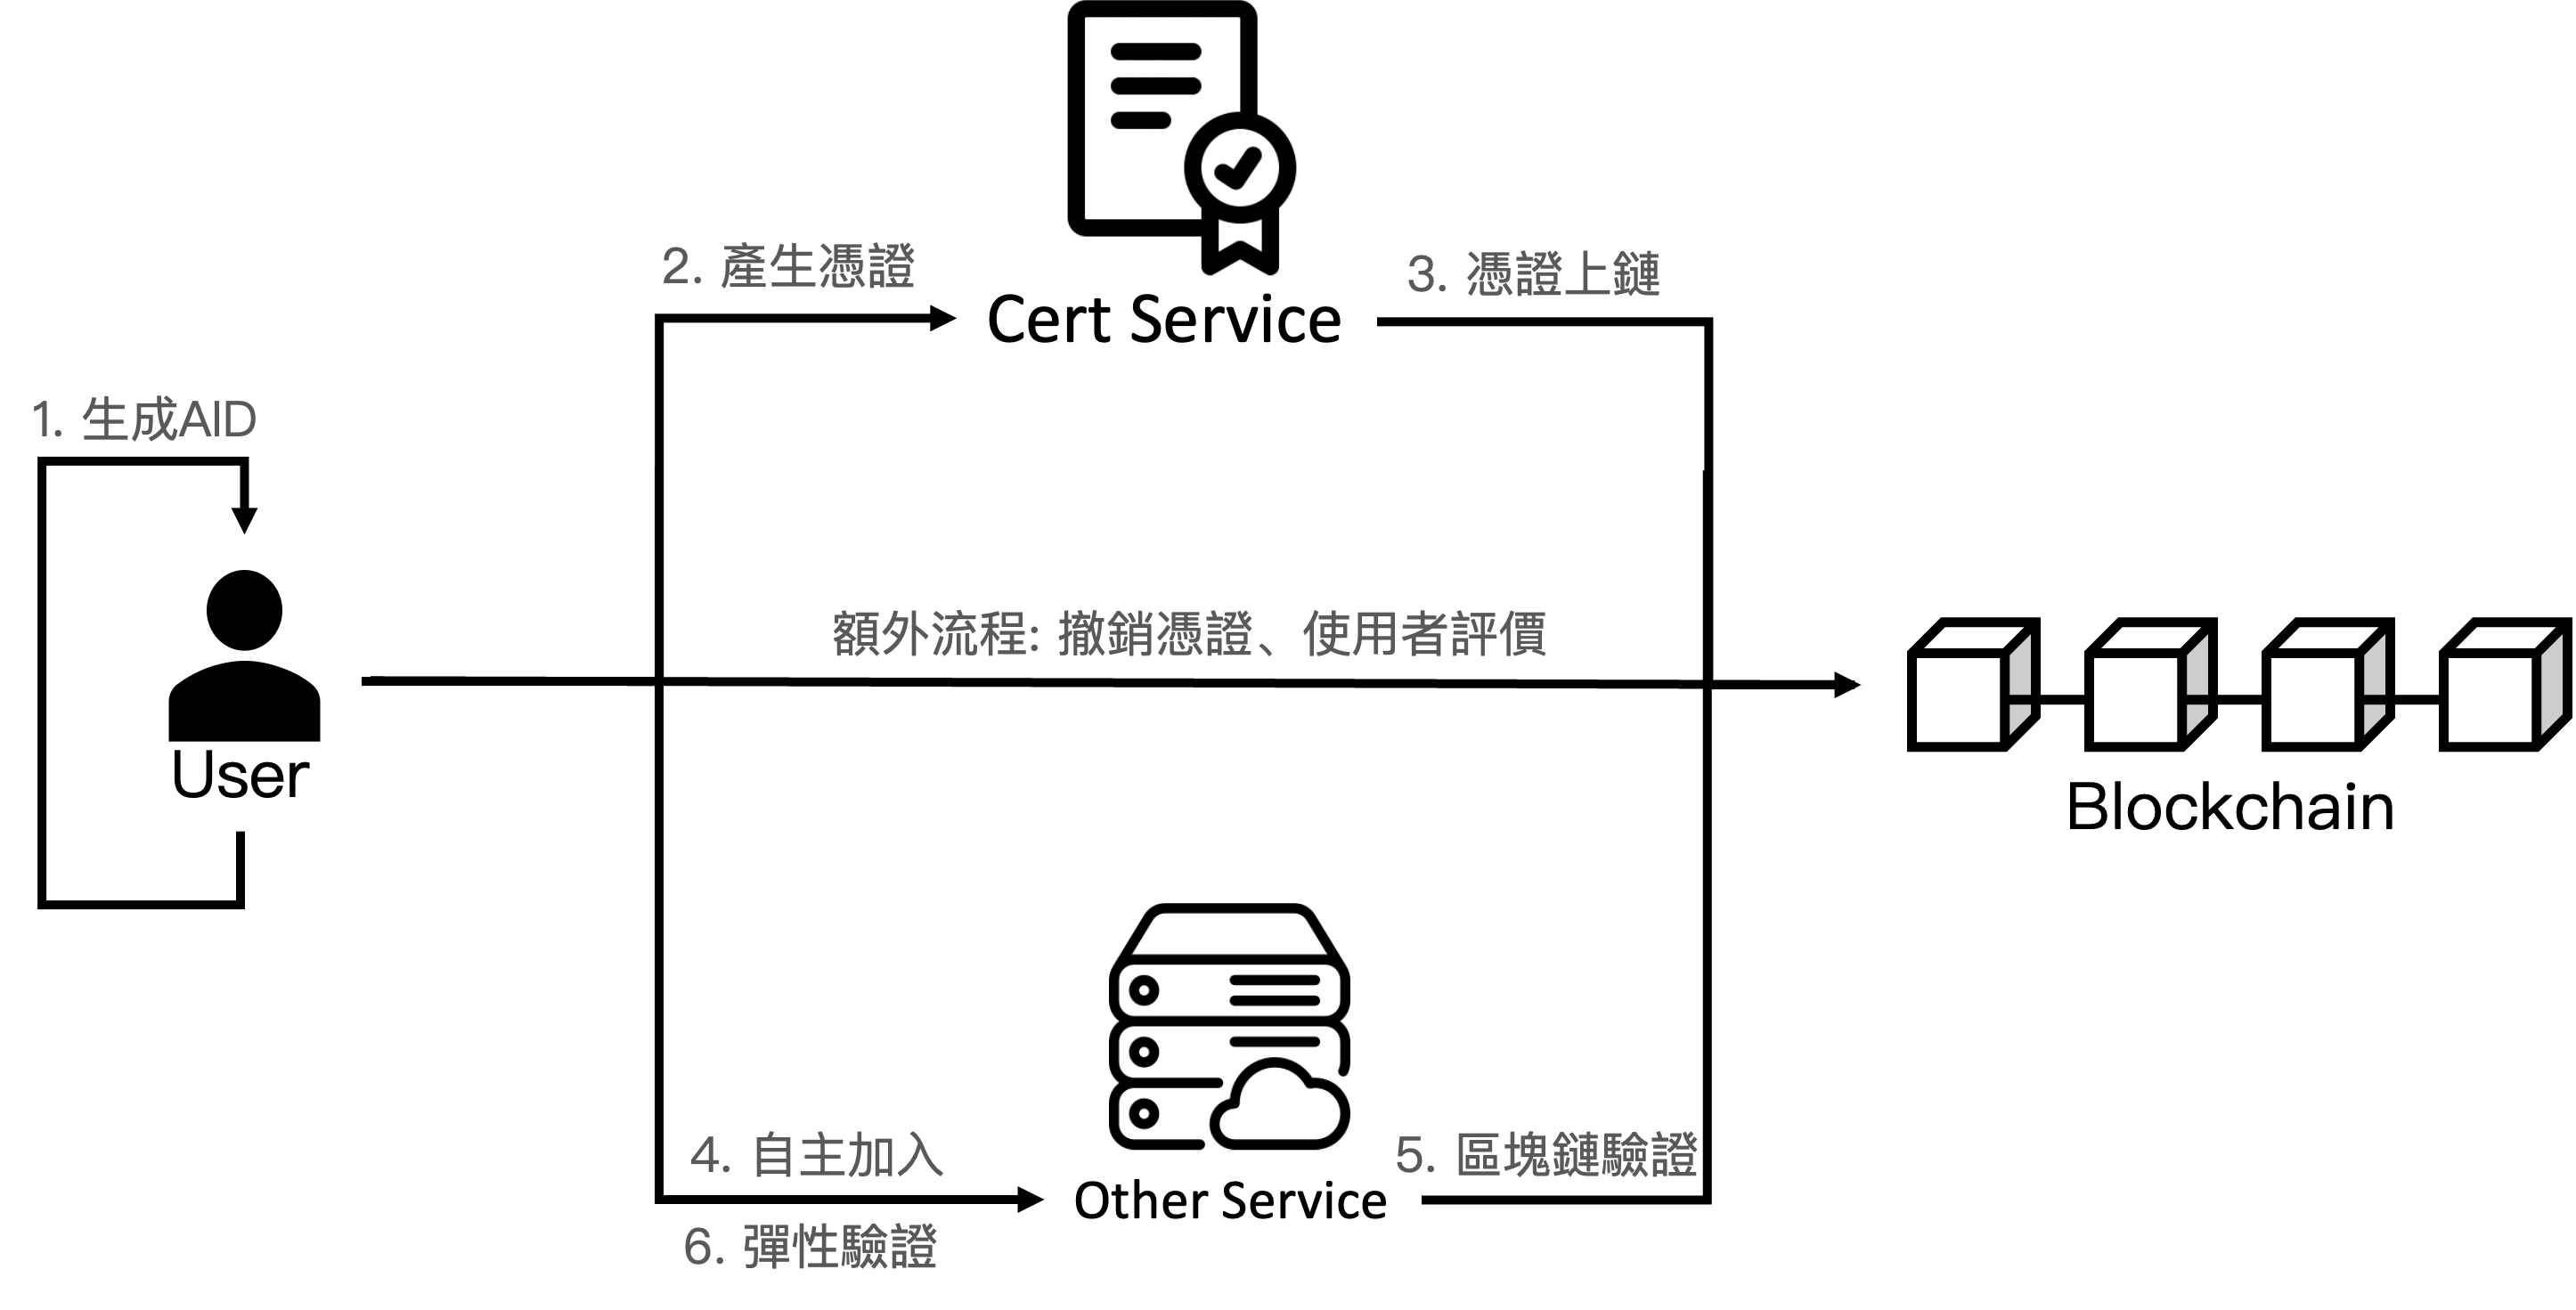
\includegraphics[width=\linewidth,keepaspectratio]{figures/flow-sc.png}
  \caption{自主證照流程}
  \label{fig:flow-sc}
\end{figure}
本研究提出的身分管理流程包含以下關鍵步驟如圖\ref{fig:flow-sc}:
\begin{enumerate}
  \item \textbf{生成AID}:透過UUID\cite{uuid}機制產生唯一編號,使用者可以根據需求設置AID內含的詮釋資料(metadata)。
  \item \textbf{產生證照}:使用者可以傳送相同的AID到不同的簽章者處建立不同目的的證照,AID內的metadata可以視情況調整。
  \item \textbf{證照上鏈}:AID的雜湊(hash)作為證照,會被簽章者記錄在區塊鏈上。
  \item \textbf{自主加入}:使用者在加入服務時,主動向服務提供者提交自己的AID,表明自己的身分。
  \item \textbf{區塊鏈驗證}:服務提供者可以在區塊鏈上取得證照得知AID的真實性。
  \item \textbf{彈性驗證}:使用者在登入服務時,可以根據AID自主選擇多因素驗證(MFA)的方式,來取得服務的信任。
  \item \textbf{使用者評價}:區塊鏈上的證照是AID的雜湊被放在智能合約中,相關參與者可以對證照進行評價,從而形成該使用者的信譽。
  \item \textbf{撤銷證照}:使用者可以隨時撤銷證照,並在區塊鏈上自行操作。這種機制可以應用於AID外流等情況。
\end{enumerate}
此外,本系統的AID除了必須的唯一識別號,支持多樣化的metadata,以下舉例說明:
\begin{itemize}
  \item 自定義多因素認證選項:滿足使用者登入的驗證所需。
  \item 選擇性資訊揭露:依照服務場景,使用者可以自行選擇要揭露的資訊。
  \item 設置證照有效期限:使用者可以設定證照的有效期限,以保護自己的隱私。
  \item 指定特定的驗證條件(如特定設備,地點或時間):增強使用者對證照的控制。
  \item 指定特定的驗證規則(設備和網路使用限制):增強使用者對證照的控制。
  \item 資源存取權限控制(如檔案存取權限):增強使用者對證照的控制。
\end{itemize}

總結來說,通過這種機制提升了系統對使用者隱私和安全的保護程度,讓使用者能夠更自主地管理其身分驗證流程,保持對個人身分驗證的控制權。
\subsubsection{數據證照}
自主身分系統中,使用者在個人設備上自行管理數據的模式引發了數據共識問題。與傳統身分系統中服務可直接調用其他服務獲取數據不同,自主身分系統在處理跨服務數據共享需求時,需要一種機制來確保數據的一致性和可信度。為此,我們擴展了自主證照的概念,提出了數據證照機制。
\begin{figure}
  \centering
  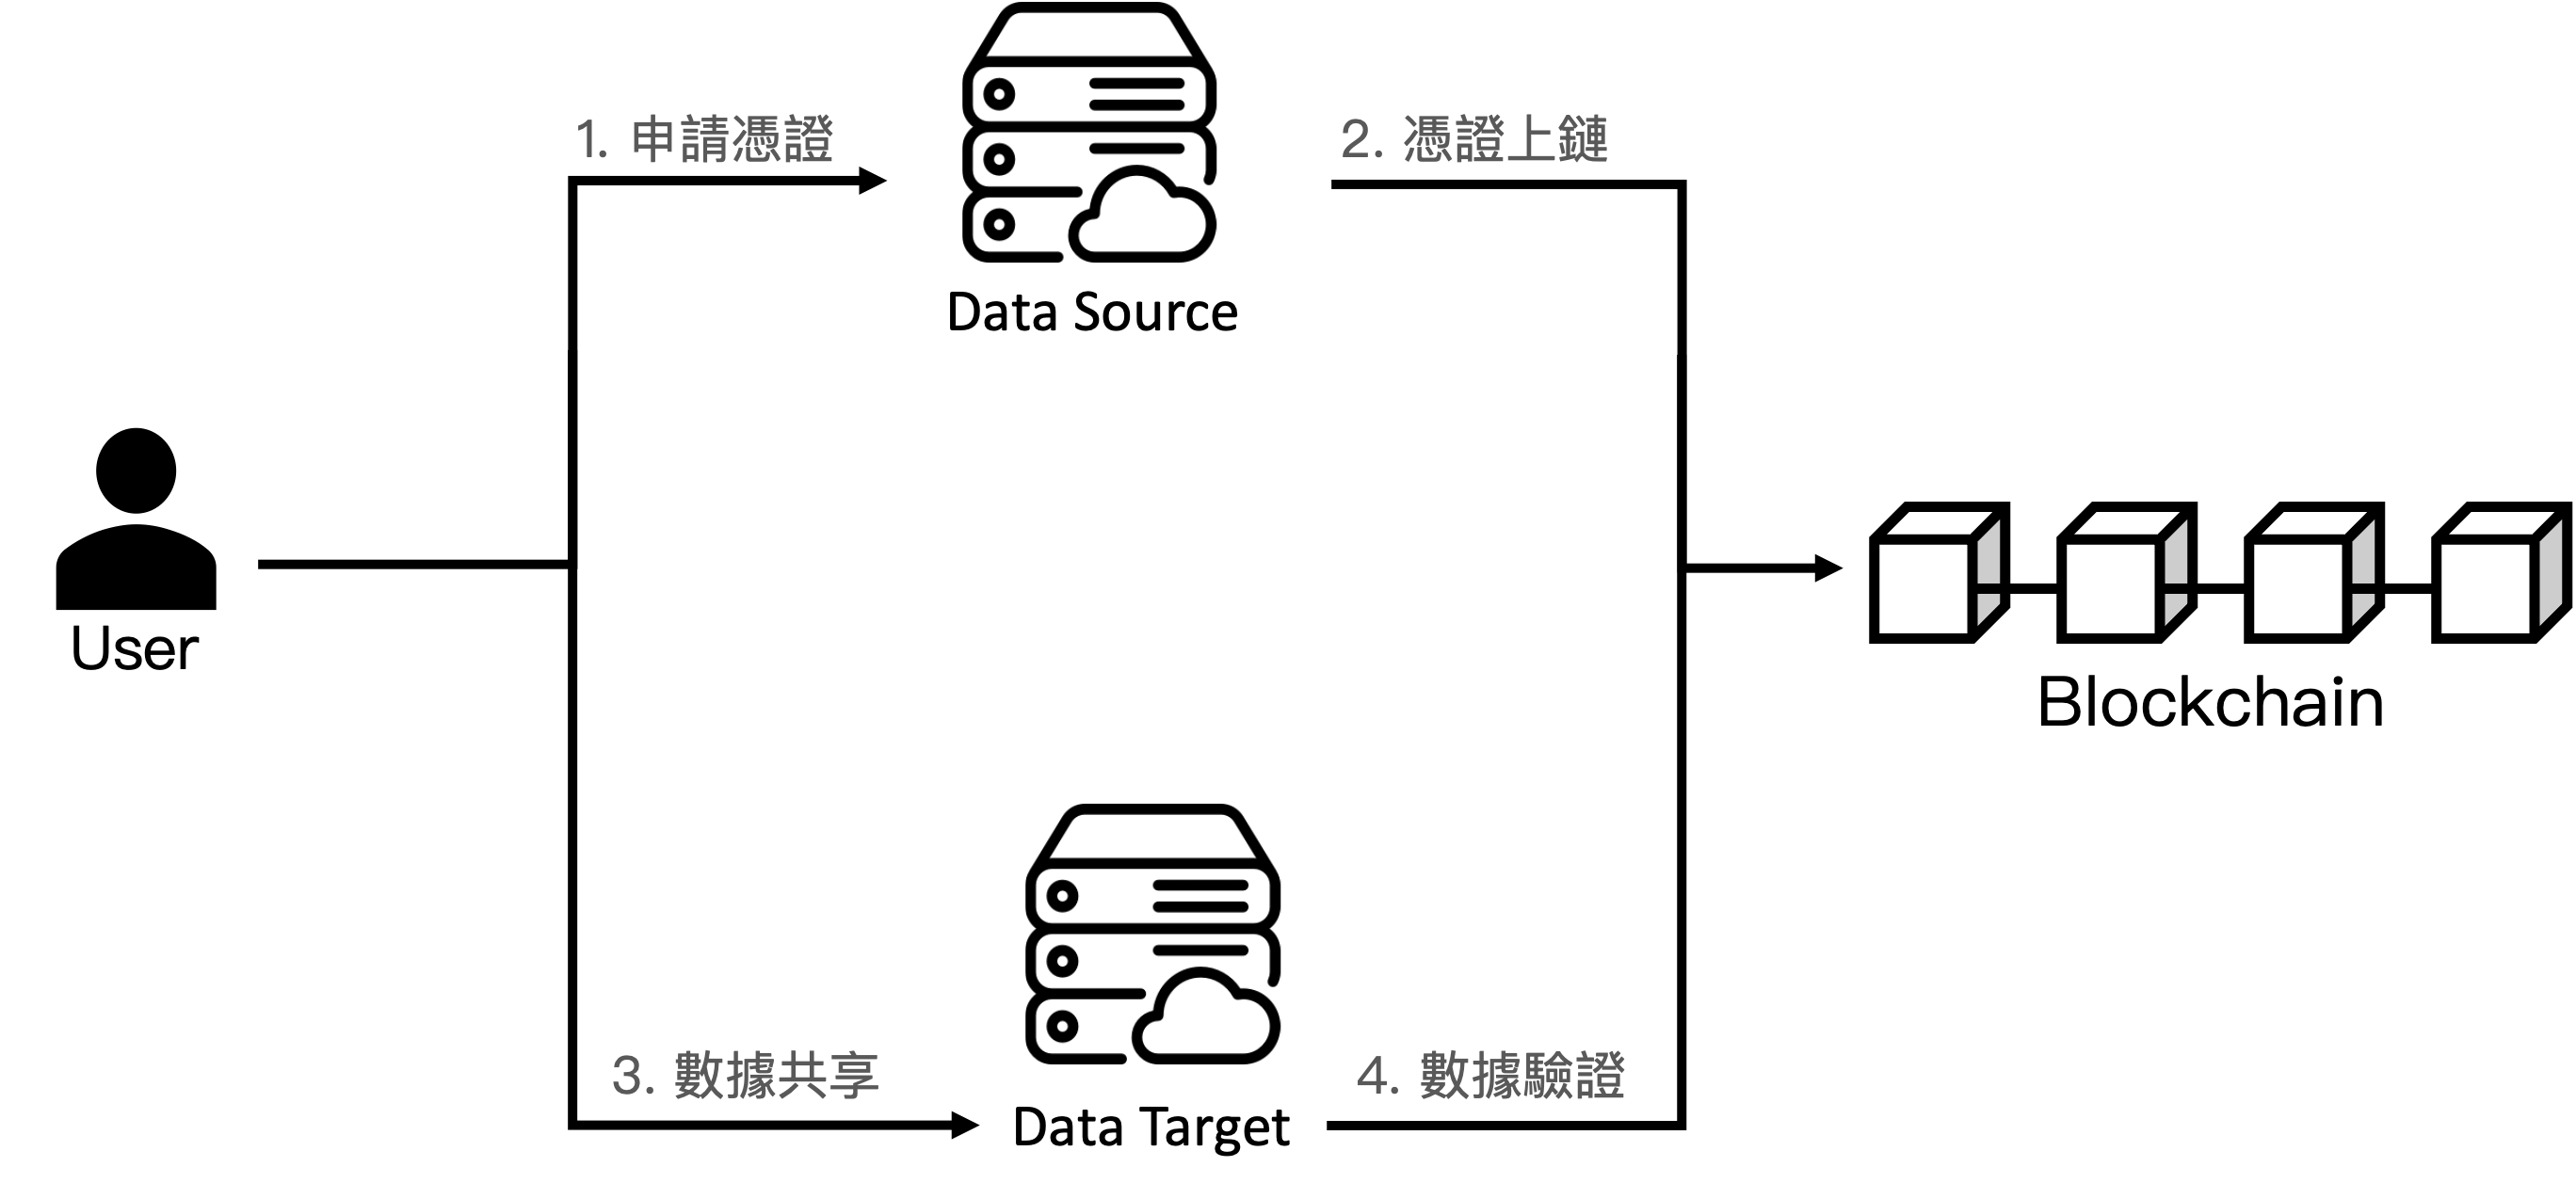
\includegraphics[width=\linewidth,keepaspectratio]{figures/flow-dc.png}
  \caption{數據證照流程}
  \label{fig:flow-dc}
\end{figure}
數據證照機制的運作方式如圖\ref{fig:flow-dc}:
\begin{enumerate}
  \item 當使用者需要向特定服務提交某個數據時,首先向能夠證明該數據真實性的其他服務提供者申請數據證照。
  \item 接受申請的服務提供者在區塊鏈上提交該使用者數據的校驗雜湊。
  \item 使用者在向特定服務提交數據。
  \item 接收數據的服務通過區塊鏈上的證照完成數據的校驗,從而確認數據的真實性。
\end{enumerate}
這種設計讓使用者能夠在不同的自主身分服務中安全地共享數據,同時向其他使用者保證數據的一致性和可信度。

此外,數據證照的雜湊被放置在智能合約中,允許相關使用者對該筆數據進行評價。這一做法將道德標準的概念從身分層面擴展到數據層面,進一步提高了數據的可信度和安全性。
\section{系統架構設計}
基於上述核心機制,我們提出了一個完整的自主身分系統架構。這個架構融合了系統的技術層次和參與者角色,形成了一個統一且高效的生態系統。本節將詳細介紹這個架構的結構和設計理念。
\subsection{系統結構概覽}
\begin{table}[h]
  \centering
  \begin{tabular}{|c|c|c|}
    \hline
    層次  & 角色    & 主要功能              \\
    \hline
    共識層 & 共識核心  & 提供可信賴的數據讀寫機制      \\
    \hline
    服務層 & 服務提供者 & 提供特定服務,不直接儲存使用者資料 \\
    \hline
    數據層 & 終端使用者 & 管理個人數據,使用服務       \\
    \hline
  \end{tabular}
  \caption{自主身分系統層次與角色對應}
  \label{tab:system-layers}
\end{table}
我們的自主身分系統架構包含三個層次,由上到下分別是共識層、服務層、數據層,每個層次對應一種關鍵角色分別是共識核心、服務提供者、終端使用者。這種對應既反映了系統的技術架構,也體現了各參與者在系統中的功能和職責。圖\ref{fig:aid-system-layer}展示了這種層次-角色對應關係,表\ref{tab:system-layers}則展示了各自的存在目的。
\begin{figure}[h]
  \centering
  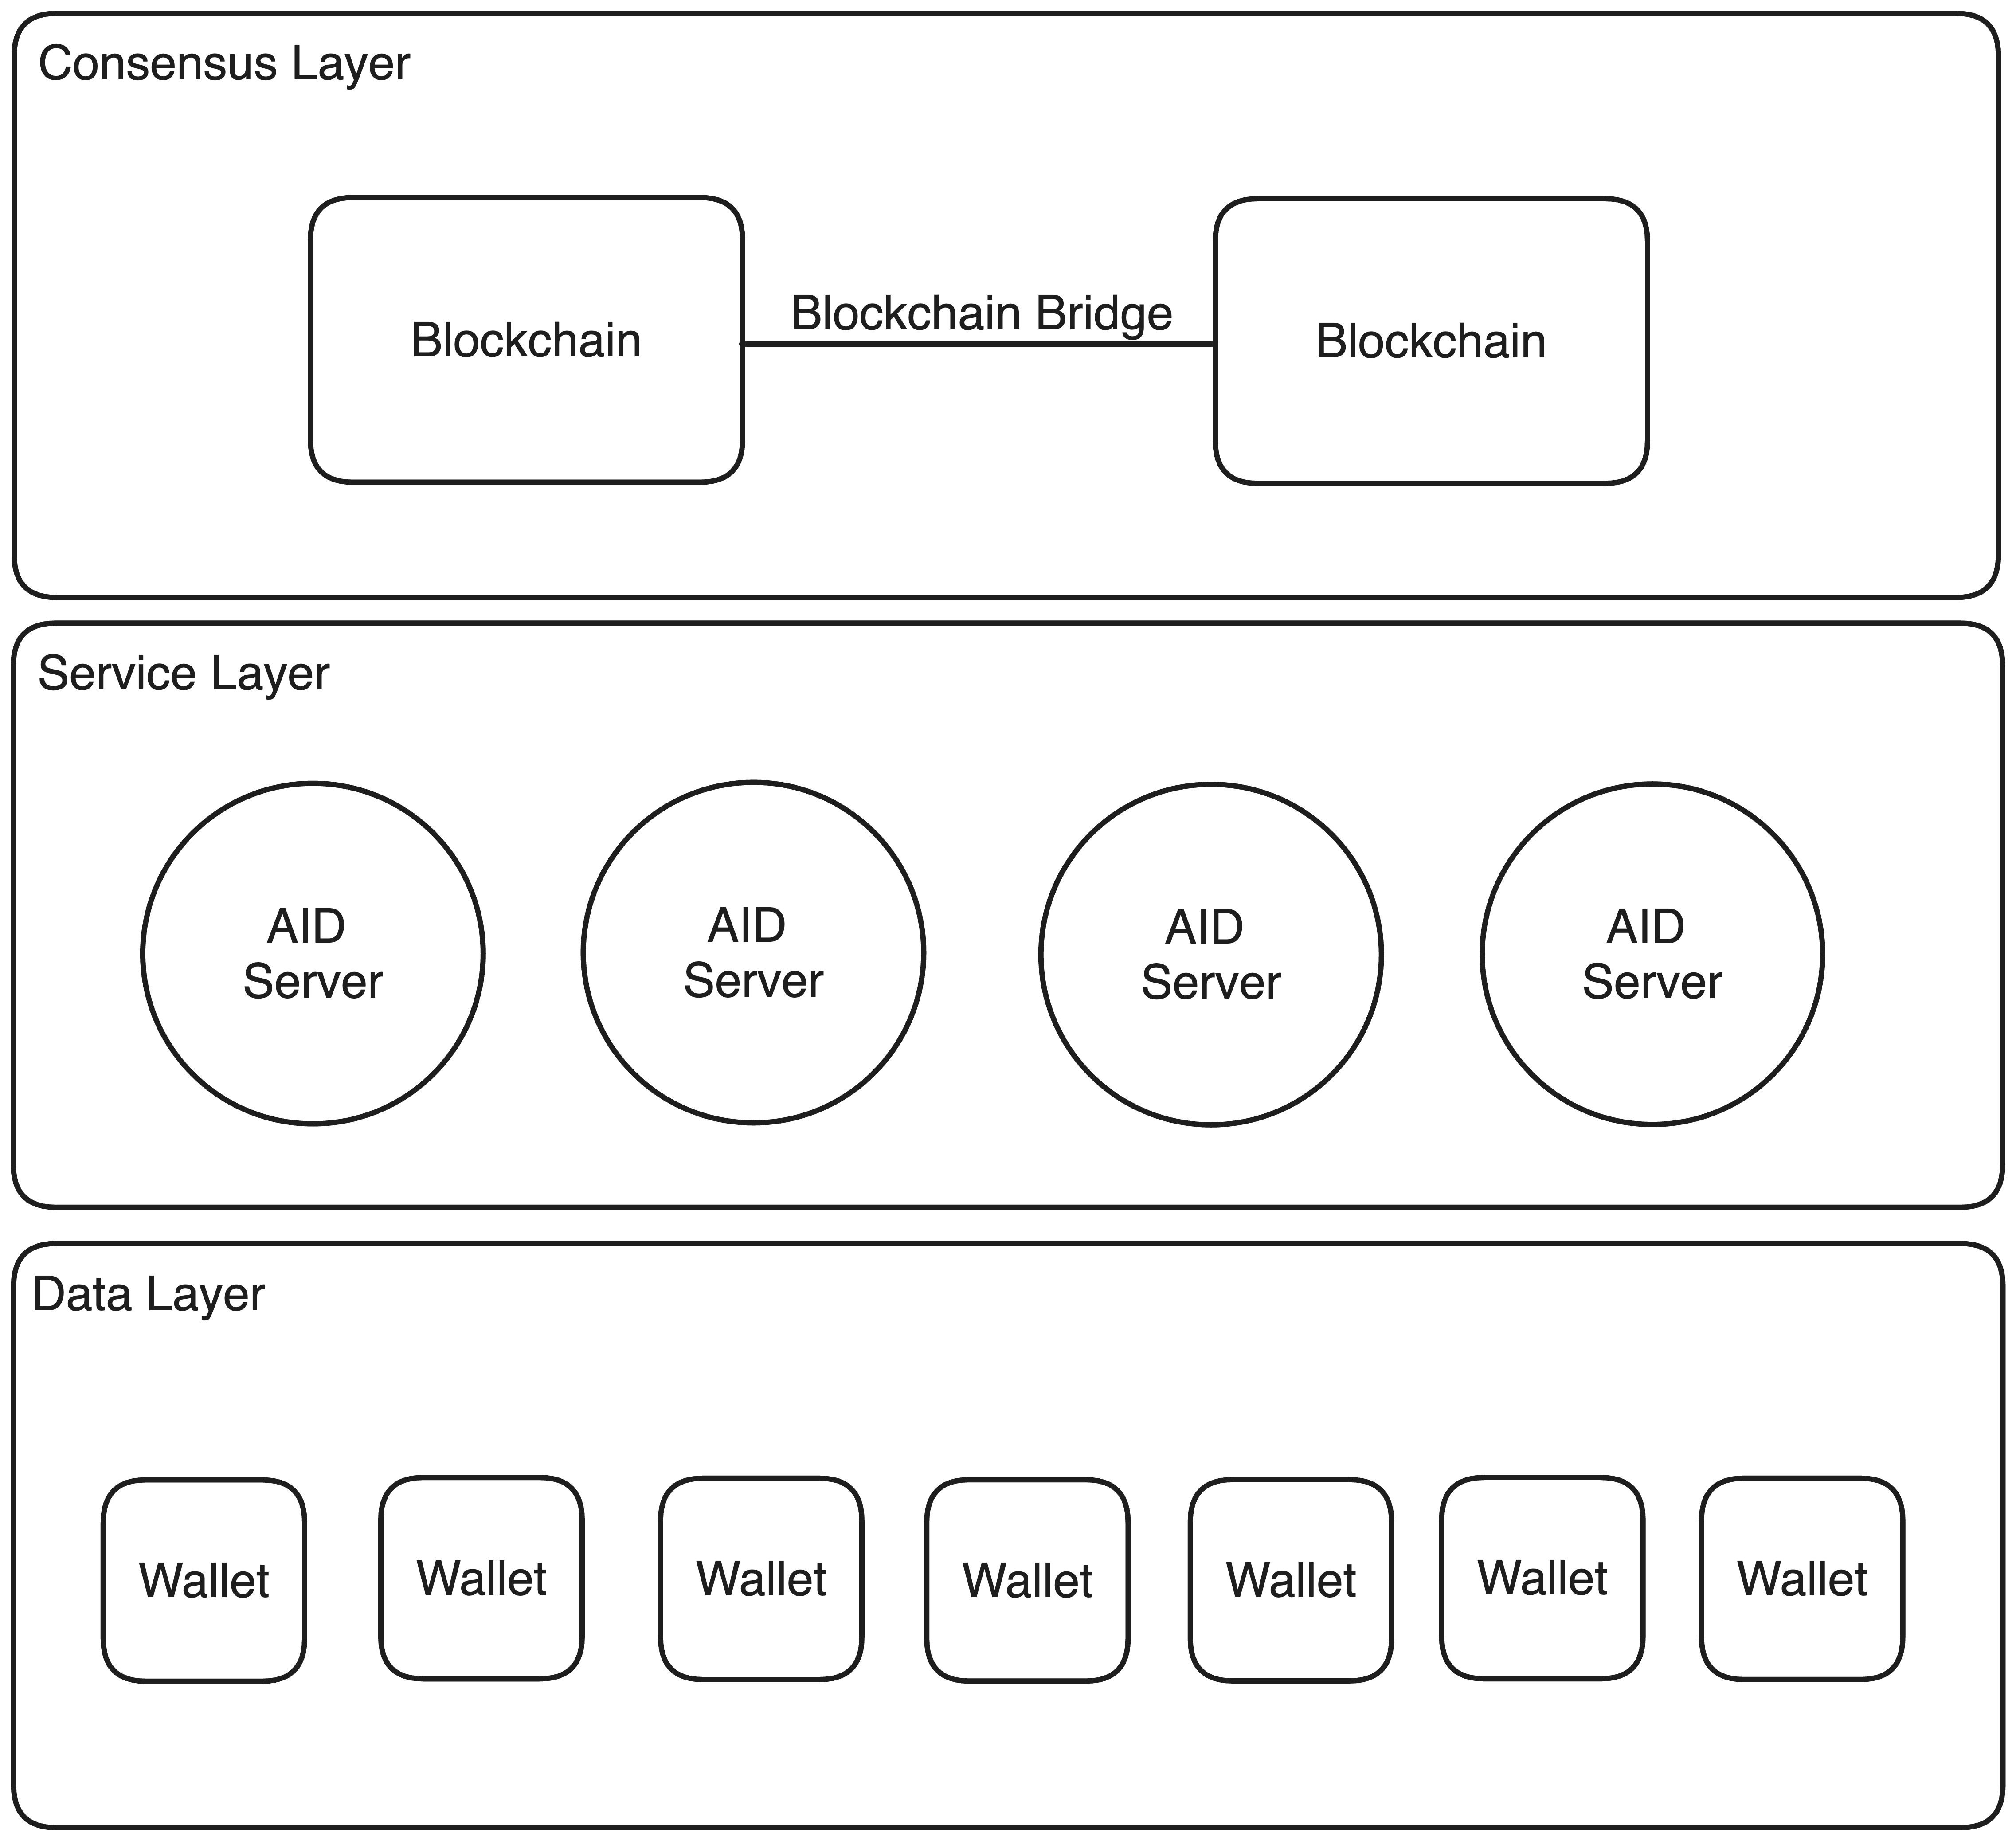
\includegraphics[width=\linewidth,keepaspectratio]{figures/aidLayers.png}
  \caption{自主身分系統結構圖}
  \label{fig:aid-system-layer}
\end{figure}
\subsection{層次與角色對應}
自主身分系統是個龐大的系統,每個層次內可以包含多個可以平行擴展的角色實作,因此為了確保各個層次能得到模組化、易抽換、可擴展、靈活、安全和互操作等優勢,我們明確訂出了各層的功能和職責。
\subsubsection{共識層與共識核心}
共識層在自主身分系統中扮演著基礎設施的角色,其主要參與者是共識核心。共識核心通過提供可信賴的數據讀寫機制,確保了「數據證照」與「自主證照」等機制在達成共識方面的可能性。其設計目的是確保數據的一致性和可信度,為整個系統提供堅實的信任基礎。共識層的實現可以靈活選擇,既可以採用區塊鏈技術,也可以使用其他形式的共識機制,以滿足不同場景的需求。
\subsubsection{服務層與服務提供者}
服務層是系統的中間層,對應的參與者是各個服務提供者。每個服務提供者都提供特定的服務,並且可以通過符合AID系統標準的介面加入系統。服務提供者不直接儲存使用者資料,而是作為使用者聚集的節點,使用者能夠自由地利用AID系統使用所需的服務。這種設計既保護了使用者數據隱私,又提供了靈活的服務串接機制。
\subsubsection{數據層與終端使用者}
數據層是系統的應用層,直接面向終端使用者。在這一層中,每個終端使用者擁有自己的數據存儲空間,並且系統提供了一個統一的數據管理介面。使用者可以自由地管理自己的數據與身分,並且通過「數據證照」與「自主證照」機制來獲得他人對個人身分或數據的信任。
\subsection{共識層}
共識層是自主身分系統的基礎建設,主要由無數個共識核心組成。共識核心內包含無數個證照,不管是「數據證照」還是「自主證照」。當共識核心由區塊鏈實作時,會使用智能合約來實現證照的寫入、讀取、更新和評價等功能,分別介紹:
\begin{itemize}
  \item \textbf{寫入:} 用於合約初始化,將數據對應的雜湊與公開資訊寫入合約狀態。
  \item \textbf{讀取:} 讀取合約狀態中的雜湊或公開資訊,用於驗證或查詢。
  \item \textbf{更新:} 由證照擁有者執行,用於即時變更證照狀態,如撤銷或停用。
  \item \textbf{評價:} 允許使用者根據智能合約規則,以特定格式讀取或寫入評價內容。
\end{itemize}
為了更好地理解共識層的運作,讓我們以學歷驗證為例。在這個場景中,使用者向學校申請學歷證明,學校將證明的數位雜湊寫入區塊鏈。任何需要驗證該學歷的服務都可以通過讀取區塊鏈上的雜湊來確認其真實性。若使用者的學歷狀態發生變化,學校可以即時更新區塊鏈上的雜湊狀態,確保驗證方獲得最新資訊。此外,如果某企業對學歷證明的可信度存疑,可以在區塊鏈上留下評價,供其他驗證方參考。

然而,這樣的設計也面臨著諸多挑戰。首要問題是如何有效評價鏈上雜湊,並將其轉化為影響使用者信譽的機制。其次,作為系統信任核心的區塊鏈,其長期穩定運營的可行性也是一個極需解決的問題。最後,在跨服務的使用者數據變化過程中,如何建立有效的共識機制同樣是一個關鍵議題。這些新架構下衍生的問題都需要深入探討和研究,以確保系統的可靠性和可持續性。
\subsubsection{評價機制}
為了解決評價問題,我們把整個自主身分系統視為一個去中心化自治組織(DAO)。基於自主身分的核心理念,我們希望每個系統參與者(包含服務供應者和終端使用者)都擁有自己的標準來基於評價判斷信譽,同時每個參與者也可以決定自己應該如何被評價。為了實現這一目標,我們提出了完整的流程來描述評價與信譽轉換:
\begin{enumerate}
  \item \textbf{產生證照:} 系統參與者創建「數據證照」或「自主證照」後,可以把對應雜湊放在自己決定的智能合約中上鏈,這個智能合約可以自訂許多規則,如是否允許別人對證照進行評價,又或是評價的格式或條件等。
  \item \textbf{產生評價:} 取得明文證照的人可以在區塊鏈上找到對應的智能合約,根據合約的規則對證照進行評價。評價的內容必須遵循智能合約的規則,否則無法上鏈。
  \item \textbf{信譽轉換:} 用有明文證照的人找到對應智能合約後可以讀取評價列表,之後根據自己認同的計算標準或演算法將評價轉換為信譽值。這個信譽值可以用於後續的信任判斷。
\end{enumerate}
進一步來說,一些使用者可能希望根據評價者的信譽值來調整每條評價的權重,以更有效地防範惡意評價。然而,設計這樣的系統並非易事。它可能需要引入評價者作為系統中的新角色,並考慮如何綜合多個評價者的評分結果\cite{josang2006exploring}。此外,還需要考慮如何通過智能合約來實現這些複雜的功能。
\subsubsection{區塊鏈的維運}
作為系統信任核心的區塊鏈如何運營,這涉及到區塊鏈的經濟模型。我們提議在區塊鏈中發行一種逐漸增加的自主身分統治代幣。這種代幣可被抵押,用於創建使用者的自主身分,藉此防止惡意使用者大規模創建惡意帳戶。每個自主身分(相當於其背後的代幣)可參與定期投票,討論評價機制的調整、新的智能合約協議等議題。為確保區塊鏈的長期運作,我們建議對失去信任的使用者實施懲罰,同時獎勵基礎設施的運作。因此,用於創建自主身分的代幣抵押後不可贖回,而是被鎖定在區塊鏈上。這樣可以確保使用者不會輕率創建自主身分,並激勵使用者維護自身自主身分的信譽。此外,我們建議對使用者在鏈上的每項操作採取使用者付費模式,使區塊鏈的維護者能獲得報酬,從而保證區塊鏈的持續運作。
\subsubsection{跨服務的狀態共識}
最後,我們需要設計一個機制來實現跨服務的使用者數據變化共識。這是一個常見的網路服務需求,如微服務間的調用即為典型案例。在我們的設計中,資料的控制權從服務提供者轉移到使用者身上,這將大幅改變當前網路後端應用的設計。基於共識層的功能,我們提議讓使用者成為多個服務之間的橋樑。具體而言,使用者在區塊鏈外傳遞特定格式的資訊,而服務提供者則在區塊鏈上驗證這些資訊,從而達成共識。
\begin{figure}
  \centering
  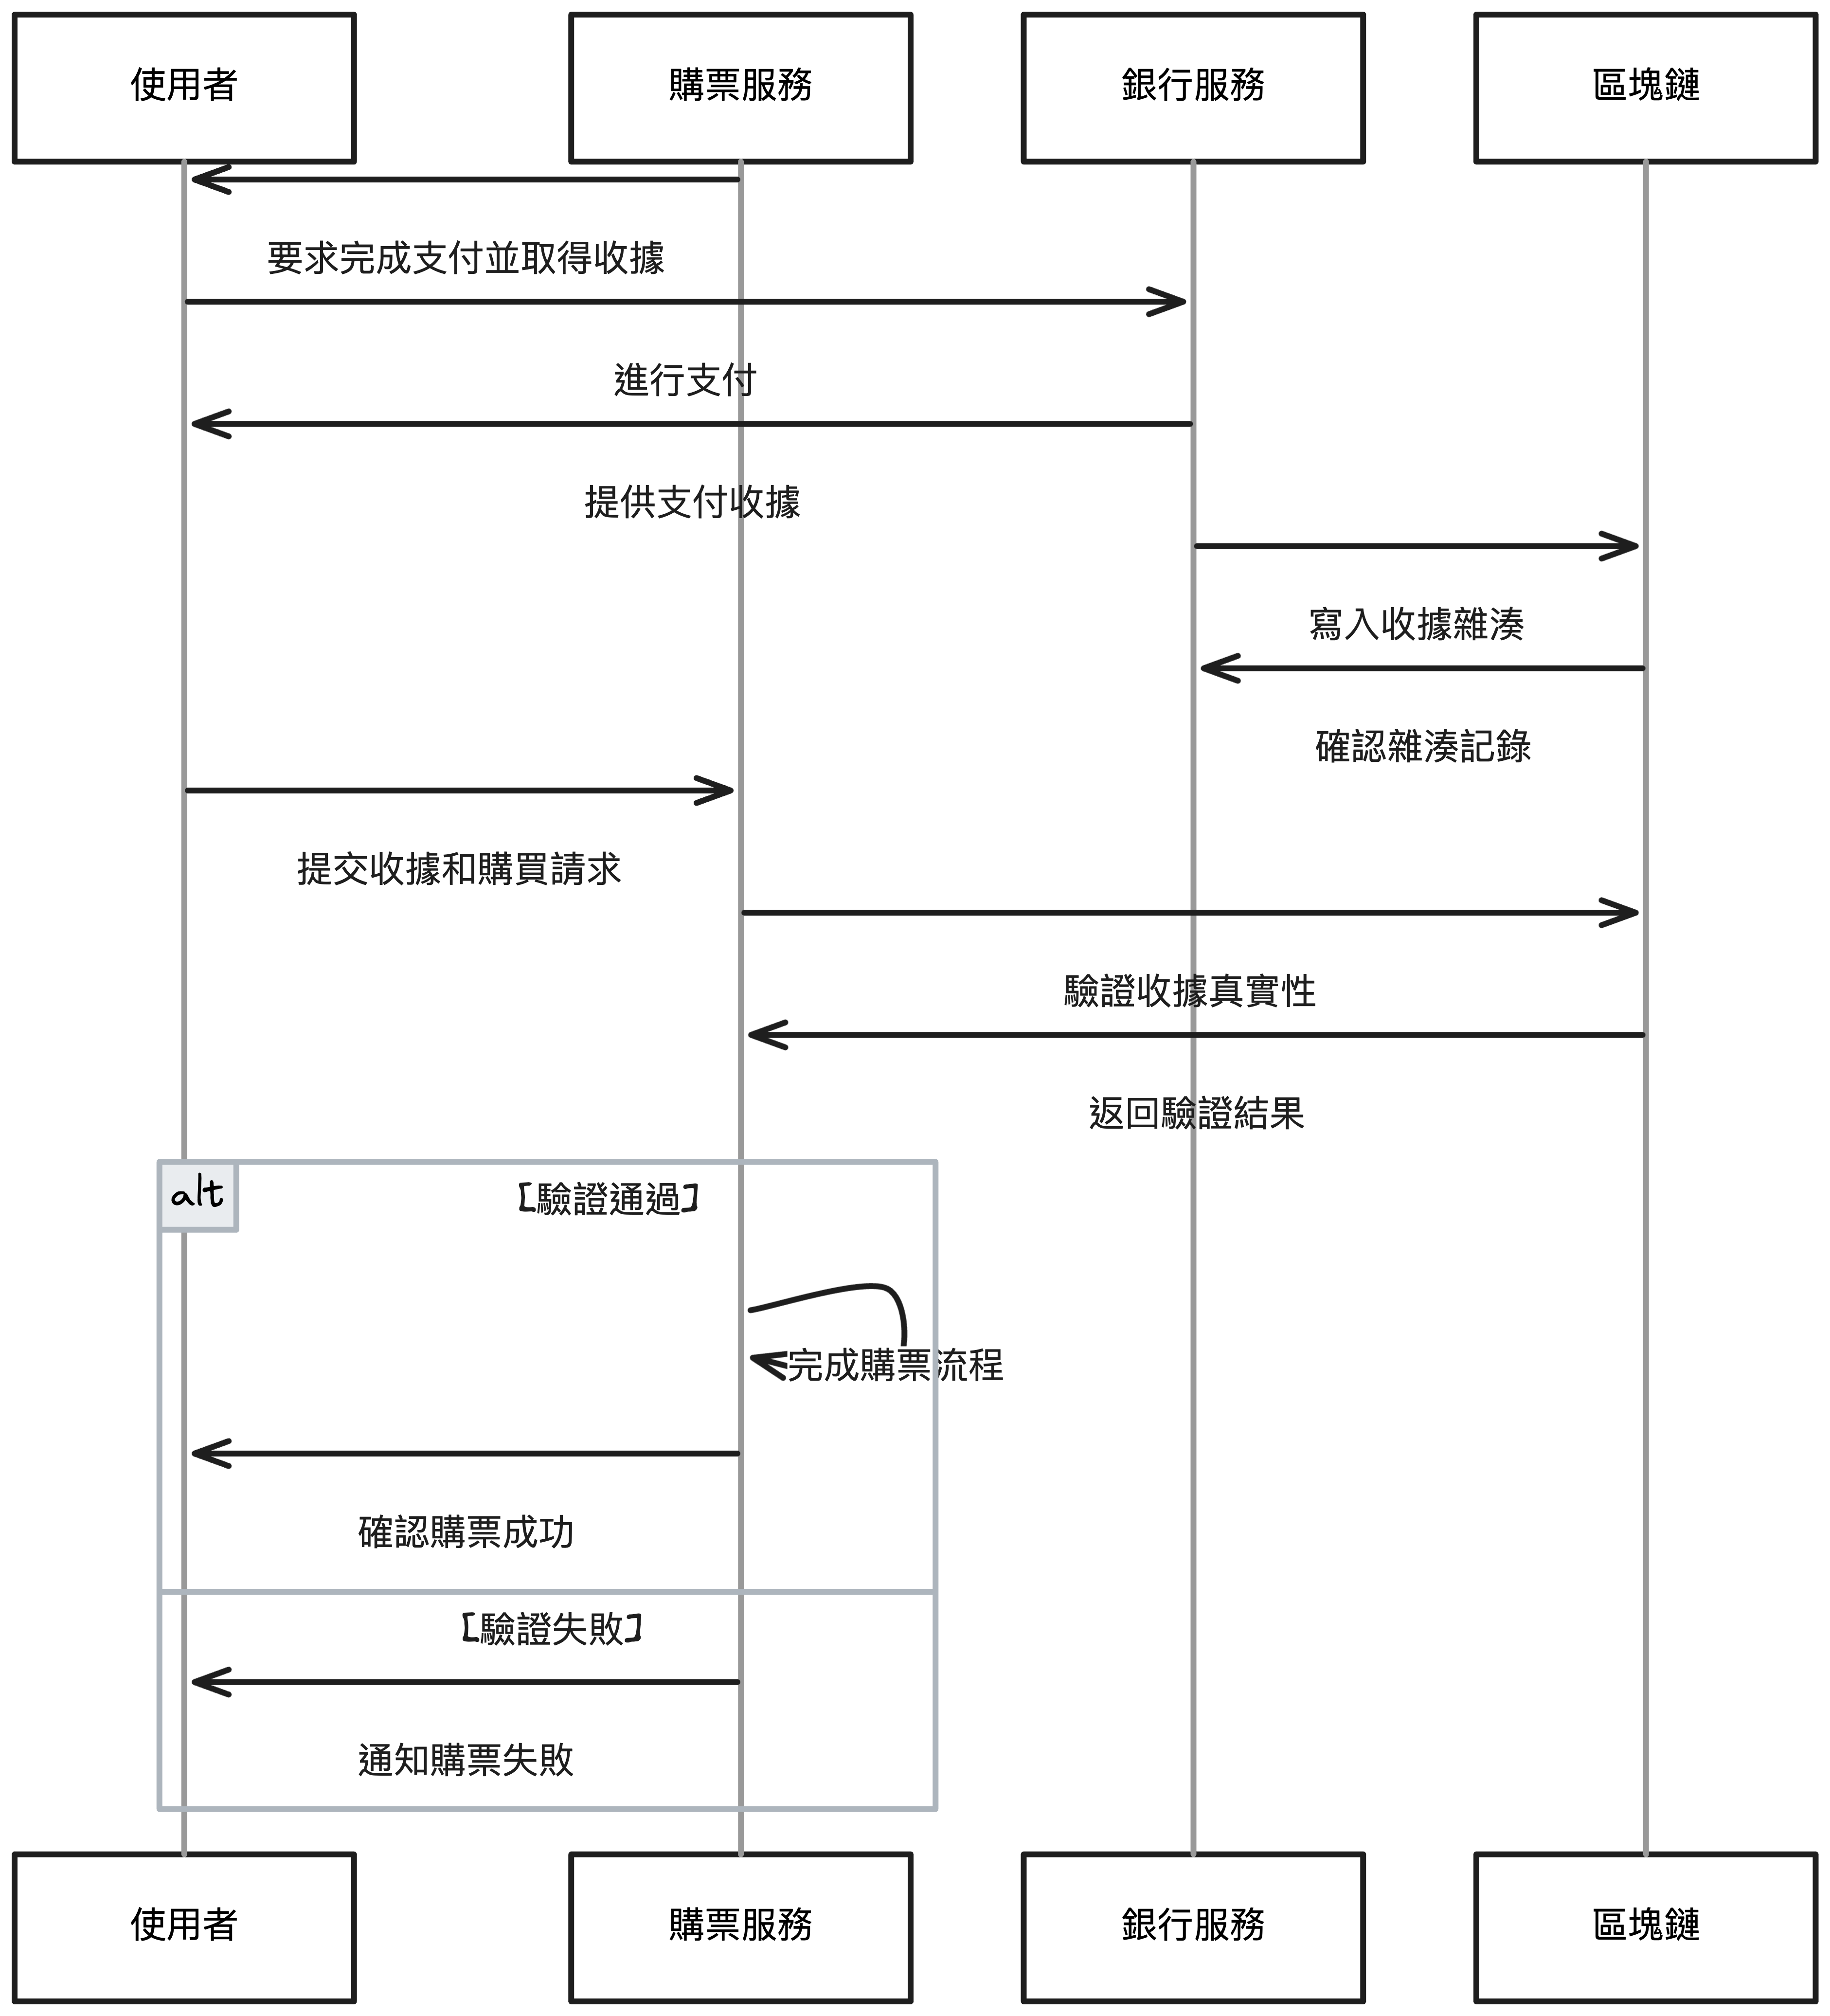
\includegraphics[width=\linewidth,keepaspectratio]{figures/flow-3-part.png}
  \caption{跨服務共識流程}
  \label{fig:flow-3-part}
\end{figure}
舉例來說,實作一個使用第三方支付服務的購票系統時,我們的方法與現行的網路後端設計有所不同。現有設計中,購票系統全權負責與支付體系的串接,使用者僅需與購票系統溝通。而在我們提出的架構中如圖\ref{fig:flow-3-part},流程如下:
\begin{enumerate}
  \item 購票系統要求使用者到銀行服務完成支付並取得收據。
  \item 銀行服務將收據的雜湊寫入區塊鏈。
  \item 使用者向購票系統提交收據和購買請求。
  \item 購票系統在區塊鏈上驗證收據的真實性。
  \item 驗證通過後,完成購票流程。
\end{enumerate}
這種方式不僅確保了數據的可信度,還賦予了使用者更多對自身數據的控制權,體現了自主身分系統的核心理念。
\subsection{服務層}
服務層是自主身分系統的應用層,負責提供各種服務。自主身分系統不包含具體服務的實作,只是提供名為AID Server的後端SDK規格,讓服務開發者能夠輕鬆地把自己的應用串接自主身分系統。我們設計了AID Server的幾個關鍵功能:
\begin{itemize}
  \item \textbf{身分管理:} 提供服務加入、登入、登出等基本身分管理功能。
  \item \textbf{證照管理:} 提供證照的創建、更新、讀取、評價等功能。
  \item \textbf{數據管理:} 提供使用者數據的導入、導出等功能。
\end{itemize}
以下將分別介紹這幾個功能的設計細節。
\subsubsection{身分管理}
對服務提供者而言,新的自主身分加入必須先由使用者上傳「自主證照」。此時,服務提供者可選擇是否接受該新自主身分。多數公開服務可能接受任何自主身分,但私人服務或有更高要求,如僅接受特定機構簽章的自主證照,或基於評價機制被充分信任的自主身分。一旦服務提供者接受新的自主身分,該身分即可開始使用服務。

為了在確保安全的同時提供便利,自主身分系統提供了兩種登入方式:簡易登入和多因素驗證登入。簡易登入是指使用者僅需提供少量資訊即可登入,如使用者別名和密碼。多因素驗證登入則要求使用者提供更多資訊,如電子郵件驗證碼、手機簡訊驗證碼或私鑰等。服務提供者可根據自身需求選擇是否啟用簡易登入功能。

另外,儘管自主身分(AID)的生成是透過UUID機制\cite{uuid}產生唯一識別號,但AID系統允許使用者在服務中設定自己偏好的別名,而非如傳統身分服務限制使用唯一的電子郵件地址作為使用者名稱。在日常操作中,系統優先讓使用者使用別名作為帳號完成簡易登入,只有當別名難以被識別時,才會要求使用者使用與UUID關聯的多因素驗證登入機制進行識別。這樣的設計我們認為更能表現出使用者對自己身分的自由控制權。

最後,服務提供者應當實作完善的登出功能,讓使用者能夠有效管理自身的在線狀態。這一功能不僅允許使用者標示自己的當前狀態,更應包含請求服務端遺忘所有數據和終止會話(session)等選項。因為在自主身分中,使用者擁有自己的數據,服務提供者僅提供服務,因此每個使用週期結束後,服務提供者應當刪除所有與該使用者相關的數據。通過提供這種全面的登出機制,服務提供者能夠進一步強化使用者對其身分資訊的掌控,同時滿足使用者在資訊安全和隱私保護方面的需求。
\subsubsection{證照管理}
服務層中的證照管理包含兩個部分:分別是「自主證照」和「數據證照」。在「自主證照」方面,大多數都是由使用者直接上傳,服務可以據此找到區塊鏈上使用者身分證照的狀態與雜湊來完成身分驗證。此外,其他實體(如服務提供者或其他使用者)可基於自身經歷,在使用者證照對應的鏈上合約中留下評價。

在「數據證照」方面,當使用者申請共享特定數據時,服務提供者可按照預定的智能合約協議創建證照,並將證照發布到區塊鏈上。如果數據發生變動,服務提供者可即時更新證照狀態,確保使用者數據的即時性和真實性。當另一個服務收到使用者在區塊鏈外提交的完整數據後,除了可以通過區塊鏈上的證照驗證數據的真實性外,還可以在區塊鏈上留下評價,為其餘服務提供者提供參考。
\subsubsection{數據管理}
因為自主身分系統的核心在於賦予使用者控制自身數據的權利,數據管理在服務層相對簡單。理論上,服務提供者的最低要求是確保使用者能夠:
\begin{enumerate}
  \item 將當次操作所必需的數據導入服務中
  \item 在操作結束後將數據導回使用者端
\end{enumerate}
然而,這種簡單設計可能大幅降低使用者體驗。例如:
\begin{itemize}
  \item 若使用者每次操作都需要導入和導出數據,許多優化使用者體驗的功能將變得不可行,因系統無法追蹤使用者歷史數據。
  \item 頻繁的大量數據導入導出會顯著增加操作延遲和網路成本。
\end{itemize}
因此,「混合數據管理」模式成為必然選擇,即部分數據由使用者保管,部分由服務提供者保管。這種設計在保護使用者隱私的同時,也確保了操作的便利性。
然而,「混合數據管理」模式仍面臨諸多需要服務提供者與使用者達成共識的問題,包括:
\begin{itemize}
  \item 哪些數據勢必要導入服務端才能完成操作?
  \item 哪些數據可以持續保留在使用者端?
  \item 服務提供者管理的數據保留時間?
  \item 數據的使用權限?
\end{itemize}
這些問題涉及對隱私和資安的權衡。為確保使用者自主權,我們建議:
\begin{enumerate}
  \item 服務層在索取數據時應提供清晰的說明,讓使用者瞭接資料上傳的必要性。
  \item 採用逐步詢問的方式協助使用者設定所有簡化的資安措施或降低的隱私保護措施。
  \item 設置應從高到低、從嚴格到寬鬆平滑過渡,使使用者能根據自身需求調整安全性和隱私保護程度。
\end{enumerate}
這種方法能在保護使用者權益的同時,為服務提供者提供必要的數據支持,實現雙方利益的平衡。透過這種「混合數據管理」模式,我們可以在自主身分系統中實現數據的高效管理,同時保障使用者的數據主權。
\subsection{數據層}
數據層是自主身分系統的存儲層,負責存儲使用者個人數據。我們設計了名為Wallet的前端SDK規格,讓數據層應用開發者能夠輕鬆地把自己的應用接入自主身分系統。Wallet的幾個關鍵功能如下:
\begin{itemize}
  \item \textbf{身分管理:} 提供自主身分的創建功能。
  \item \textbf{數據管理:} 提供使用者數據的上傳、下載等功能。
  \item \textbf{證照管理:} 對共識雜湊的更新、讀取、評價等功能。
  \item \textbf{數據存儲:} 儲存使用者的數據。
\end{itemize}
以下將分別介紹這幾個功能的設計細節。
\subsubsection{身分管理}
Wallet 的身分管理主要提供一個核心功能:創建自主身分。這裡的創建並非指使用者加入某個服務,而是包含兩個主要功能:
\begin{enumerate}
  \item 使用者直接在本地裝置透過隨機產生的UUID創建自己的自主身分
  \item 透過「自主證照」機制創建新的證照
\end{enumerate}
在我們的設計中,使用者可依據需求使用個人裝置創建不同的AID,並為不同需求生成不同的身分證照,再利用這些證照證明AID的真實性。當使用者需要向服務證明自己是AID的真實持有者時,僅需透過Wallet完成AID上標示的多因素驗證方案。
\subsubsection{數據管理}
Wallet的數據管理功能主要在服務需要時,將特定數據自主上傳至服務中,並在服務結束後自主下載回本地裝置。這裡的「自主」指使用者可自由選擇是否上傳或下載數據,並可自由選擇上傳或下載的數據內容。這樣的設計不僅更徹底地保護了使用者的安全與隱私,更因為由使用者自行攜帶數據在服務間移動,而徹底解決了數據孤島的問題。
\subsubsection{證照管理}
Wallet的證照管理功能主要對共識層內證照進行更新、讀取、評價等操作。基於「數據證照」與「自主證照」機制,使用者與服務需要在共識層中的區塊鏈上基於智慧合約留下AID雜湊,讓人們可在區塊鏈上驗證AID的真實性。此外,所有使用者(包含服務提供者)都可在區塊鏈上對智能合約進行操作,以留下評價,藉此形成共識達成信任。

在Wallet中實作的證照管理功能,使用者可輕易從Wallet中直接讀取共識層內的信任關係,並直接在共識層中更新自己身分證照的狀態,以及對他人或服務的證照評價。這樣的設計不僅提高了使用者的自主權,更讓使用者能更直接地參與共識層的運作。
\subsubsection{數據存儲}
Wallet的數據存儲功能主要用於儲存使用者的各類數據,包括證照、公私鑰、個人資料以及與各服務的交互紀錄等。這種設計使 Wallet成為使用者的個人化數據中心,實現統一管理。然而,將個人移動設備轉化為數據中心需解決備份、遷移和雲端儲存等問題。雖然我們鼓勵使用者自主選擇解決方案,但仍提供以下建議實作:

每個採用自主身分系統的應用都應包含Wallet模塊,並利用設備的嵌入式資料庫存放數據。使用者可設置各Wallet的同步策略,包括自動同步(按需獲取數據)、完全同步(複製全部使用者數據)和手動同步(使用者指定數據複製)。這種設計便於實現備份、遷移和雲端儲存等功能,提升使用者數據管理的便利性。具體實現概念如下:
\begin{itemize}
  \item \textbf{遷移:} 新 Wallet 可通過手動輸入舊 Wallet 的公開地址或直接連接同一設備上的已啟動 Wallet 來建立連結。遷移後,新 Wallet 可設置對舊 Wallet 的同步策略。
  \item \textbf{雲端儲存:} 考慮到在單一移動設備上存儲全部個人數據的安全風險,以及終端使用者難以維護家庭點對點(Point-to-Point,P2P)集群的現實,專業雲端服務供應商可提供執行完整Wallet的服務。使用者支付費用後,可讓其他 Wallet連接到此雲端Wallet。
  \item \textbf{備份:} 當使用者在多個設備上維護多個Wallet,並重複存儲每項數據時,自然形成了數據備份機制。
\end{itemize}
這種多元化的數據管理策略不僅提高了數據安全性,也增強了系統的靈活性和使用者體驗。
\section{資安與隱私議題}
自主身分系統不僅僅要提供卓越的功能,我們還希望能在確保使用者體驗的同時,保護使用者的隱私和資訊安全。為此,我們提出了一系列的資安與隱私議題,並提出了相應的解決方案。
\subsection{身分識別問題}
以自治身分為例,為了確保身分系統的去中心化,大幅度使用了區塊鏈相關技術,卻因此導致使用者體驗大幅度偏離一般使用者的需求。我們為了解決這個問題,在自主身分系統的共識層中定義了兩種登入方法:簡易登入和多因素驗證登入。期望可以根據不同情境,讓使用者選擇登入方式,以同時滿足安全性和便利性的需求。

但是,系統該如何確保使用者能使用簡易登入方式呢?畢竟簡易登入可能因提供資訊不足而被攻擊者冒充或無法成功辨識身分。為此,我們提出了「基於使用者時空的分析方法」,通過追蹤使用者每次操作時夾帶或產生的資訊來辨識使用者身分,並配合「基於危險程度的驗證機制」找出應要求多因素驗證的時機。

接著我們會詳細介紹「基於使用者時空的分析方法」與「基於危險程度的驗證機制」這兩種特殊解決方案。
\subsubsection{基於使用者時空的分析方法}
每個身分本質上可視為一個隨時間變化的動態向量空間,其維度可謂無窮。每次對使用者的身分驗證都可視為取得特定時間僅含部分維度的向量。這方法的核心是讓使用者自主決定提供哪些維度,並在每次與系統互動時攜帶這些資訊。基於此概念,即讓使用者使用簡易登入,只要使用者自動攜帶裝置指紋、位置等資訊,系統即可通過比對這些資訊來進一步確認使用者身分。
\begin{enumerate}
  \item 使用者i在時間t的身分向量:
        \begin{equation}
          \mathbf{i}(t) = (i_1(t), i_2(t), \ldots, i_n(t), \ldots), \quad n \to \infty
        \end{equation}
  \item 使用者i在時間k登入時傳入的向量:
        \begin{equation}
          \mathbf{v}_k = (v_{k1}, v_{k2}, \ldots, v_{km}), \quad m \ll n, \quad v_{kj} = i_j(t_k) \text{ 對某些 } j
        \end{equation}
  \item 暫存的向量集合(假設 $\dim V = m$):
        \begin{equation}
          \mathbf{v}_k = (v_{k1}, v_{k2}, \ldots, v_{km}) \in V, \quad \dim V = m \ll n
        \end{equation}
  \item 假設相似度函數為s:
        \begin{equation}
          s: \mathbb{R}^m \times \mathbb{R}^m \to [0, 1]
        \end{equation}
  \item 身分推測方法:
        \begin{equation}
          \text{Identity} = \arg\max_{\mathbf{v}_i \in V} s(\mathbf{v}_{\text{new}}, \mathbf{v}_i)
        \end{equation}
\end{enumerate}
舉例來說:使用者在某次登入時提供了自己的別名、性別、所在地區等資訊,而在下次登入時僅提供了性別、所在地區等資訊,系統可以通過比對這兩次向量來推測使用者的別名。這種方法使使用者在不提供完整資訊的情況下,仍能通過部分資訊完成身分驗證。

然而,這種方法也帶來了一些問題。例如,使用者提供的維度多寡會影響系統的準確性,甚至使用者提供的維度是否包含可變資訊會影響系統的安全性。因此,我們提出維度的選擇甚至各個維度的權重應由使用者自主決定,而系統僅提供推薦機制。這樣可讓使用者在不同情境下使用不同方法,以滿足其需求。
\subsubsection{基於危險程度的驗證機制}
AID系統允許使用者自定義各種行為的危險程度,並據此調整驗證的嚴謹度。然而,這種設計可能帶來兩個極端問題:過高的嚴謹度可能導致正常登入受阻,而過低則可能危及系統安全。為此,我們提出「基於危險程度的驗證機制」希望系統性地協助使用者為不同場景設定合適的驗證嚴謹度。

這個機制建立在「基於使用者時空的分析方法」之上,綜合考慮三個關鍵因素:行為的危險程度、符合的維度數量,以及時間點的接近程度。這三者的互動決定了所需的驗證嚴謹程度。簡而言之,行為越危險,需要越嚴格的驗證;而越嚴格的驗證,則要求更多的維度符合和更接近的時間點。

值得注意的是,我們的系統中,使用者可以自主決定行為的危險程度,系統僅提供建議。這種設計能滿足不同情境下的需求。例如,對於個人銀行帳戶,使用者可能將所有行為視為高度危險,因此需要最嚴格的驗證。相反,對於社群媒體帳戶,閱讀文章可能被視為低風險行為,而發布內容則可能需要更嚴格的驗證。

我們建議使用者將危險程度定義為對數據操作的敏感度:越敏感的數據越危險,越危險的數據則需要越嚴謹的驗證機制。通過這種方式,我們希望為各種使用場景提供既靈活又安全的身份驗證解決方案。
\subsection{密碼救援問題}
密碼救援問題是自主身分系統中的一個重要問題。在傳統身分系統中,密碼救援通常是通過中心化的機制來實現的,其本質的概念就如同系統內存在著一位管理者,共同管理著使用者的身分。但這明顯違背了自主身分追求的價值觀,因此我們提出了「極致多因素認證」的概念。

允許使用者在創建自主證照時設置多種驗證方案,包括難以遺失或忘記的方法,如生物特徵識別(指紋或臉部辨識)。如此,即便使用者忘記密碼,亦可通過這些驗證方式重新取回身分。進一步擴展此方案,我們還可以將「極致多因素認證」概念應用於「基於危險程度的驗證機制」,根據危險程度要求使用者使用多種方法完成多因素驗證,進一步提高安全性,讓使用者即使已經被攻擊者奪取身分,也能通過補充更多項驗證的方式來取回身分。
\subsubsection{極致多因素認證}
傳統身分驗證系統中,多因素認證主要被視為登入時的固定驗證方案。然而,在自主身分系統的設計中,為了實現使用者功能的自由管理,我們需要一種更靈活、更強大的驗證機制,以取代傳統系統中系統管理員的角色。為此,我們提出了「極致多因素認證」的概念。
這一新概念的核心在於:不再將特定的多因素驗證方法視為使用者登入的唯一途徑。相反,從服務器的角度來看,每個驗證因素都應被視為使用者向服務器自主證明身分的一種方法。這種方法的靈活性體現在:
\begin{itemize}
  \item 在高風險情況下,系統可能要求連續多種因素的驗證以確保安全。
  \item 在低風險環境中,可能僅需一種因素即可完成驗證。
  \item 即便使用者遺失了某個重要的驗證因素,系統也不應將其視為無法登入,而是要求提供更多其他因素的驗證來補償。
\end{itemize}
通過這種動態和適應性的方法,極致多因素認證不僅提高了系統的安全性,還增強了使用者的身分管理自主權,為自主身分系統提供了一個更加靈活和強大的驗證框架。
\subsection{被遺忘權}
雖然在自主身分系統中,由使用者的個人裝置管理所有數據,但這並不意味解決了被遺忘權的問題。實際上,不管是使用者與他人互動後其他人存下的數據亦或是單純為某個行為的日誌,都不太可能被完全遺忘。爲此,我們提出當使用者希望遺忘數據時,除了直接清除個人保留的數據,還能讓其他人無法再利用這些數據指向使用者本身。因此不管是「數據證照」還是「自主證照」都確保了區塊鏈中僅保留雜湊,而不保留數據本身。理論上,服務內部不會存儲使用者數據;即使確實存儲了,在自主身分中唯一能證明數據擁有人的是使用者本身,因此相當於使用者與數據無關。這個概念類似於Cameron\cite{cameron2005laws}所描述的單向身分:使用者可以通過個人證明指向自己的數據,但僅有數據無法指向使用者。
\subsection{積極數據授權}
從近年來的GDPR研究中就可以發現,積極數據授權是最多大型企業所面臨的難題。在自主身分系統中,各個服務一樣也會經手使用者的數據,因此我們也提出一個機制來解決這個問題。這個機制的核心在於:使用者與服務提供者之間的數據授權應該是明確的,公平的。

透過數據層的API與服務互動時,使用者與服務應該使用「數據證照」來明確定義數據的內容與授權,。使用者與服務都應該要留存該證照,並在區塊鏈上留下雜湊。這樣,當數據被濫用時,使用者可以通過公開證照證明數據被濫用,反之,服務提供者也可以通過公開證照證明數據被合法使用。這樣的設計讓使用者與服務提供者之間的數據授權變得更加明確且公平。
\section{資料結構}
我們會分別介紹自主身分系統中各角色重要物件的資料結構,以此讓讀者更清晰的了解系統的設計。
\subsection{共識核心}
共識層由不同的智能合約組成,每個智能合約都有自己的資料結構。這裡我們將介紹「自主證照」和「數據證照」機制所需智能合約的參考資料結構。
\begin{itemize}
  \item \textbf{自主身分唯一編號:} 透過UUID生成,用於識別使用者,此欄位在重視隱私的情況下可不填。
  \item \textbf{證照操作公鑰:} 對應私鑰被註記在明文證照中,因此智能合約可以確保操作者真的有得到實際的證照。
  \item \textbf{證照雜湊:} 擁有明文證照的系統使用者可以藉此完成證照真實性的驗證。
  \item \textbf{證照狀態:} 用於記錄證照的當前狀態,可能包括「正常」、「失效」、「遺忘」等。
  \item \textbf{證照評價:} 用於記錄證照的評價,可能包括「好」、「壞」、「中立」等,並且同時可以紀錄評價者的AID。
\end{itemize}
\subsection{AID Server}
服務層中一般會暫存使用者的明文證照與關聯服務商業邏輯的資料結構,我們這裡僅介紹明文證照的參考資料結構。
\begin{itemize}
  \item \textbf{自主身分唯一編號:} 透過 UUID 生成,用於識別使用者。
  \item \textbf{證照操作私鑰:} 對應公鑰被註記在智能合約中,因此智能合約可以確保操作者真的有得到實際的證照。
  \item \textbf{簡易識別方案:} 列出使用者想要使用的簡易登入方案與對應辨識內容,如「帳號密碼」、「IP綁定」等。
  \item \textbf{多因素驗證方案:} 列出使用者想要使用的多因素驗證方案與對應辨識內容,如「簡訊驗證」、「硬體金鑰」等。
  \item \textbf{個人資訊:} 用於揭露使用者願意提供的個人資訊,如「姓名」、「性別」等。
  \item \textbf{服務設定:} 用於記錄使用者希望自主設定的內容,如證照的權限、有效期等。
\end{itemize}
拿簡易識別方案舉例,明文證照就會包含「帳號」與「密碼」兩個欄位,而「IP綁定」則會包含「IP位址」欄位。多因素驗證方案的資料結構也類似,如「簡訊驗證」會包含「手機號碼」欄位。

另外,為了確保簡易登入的安全性,我們也建議服務提供者暫存使用者每次識別空間與對應時間,以便透過「基於使用者時空的分析方法」來識別使用者。接著提供我們建議的暫存資料結構。
\begin{itemize}
  \item \textbf{使用者身分:} 自主證照明文。
  \item \textbf{使用者時間:} 用於記錄使用者每次識別的時間。
  \item \textbf{使用者空間:} 用於記錄使用者每次識別所拿到的所有數據,包含裝置指紋、IP位址等。
\end{itemize}
\subsection{Wallet}
數據層中一般會存儲使用者的所有數據,我們將介紹所有數據的參考資料結構。
\begin{itemize}
  \item \textbf{自主身分列表} 同一個Wallet可以管理多個AID。
        \begin{itemize}
          \item \textbf{自主身分唯一編號:} 透過UUID生成,用於識別使用者。
          \item \textbf{證照列表:} 用於記錄AID的所有證照明文。
          \item \textbf{使用者個資:} 用於記錄AID的所有個人資訊。
          \item \textbf{使用者密鑰:} 用於記錄AID的所有公私鑰。
          \item \textbf{使用者數據:} 用於記錄AID在所有服務中的數據,以列表的形式存在,可以用服務的AID來索引。
        \end{itemize}
\end{itemize}
\section{本章總結}
為了全面評估自主身分系統相較於傳統身分系統的優勢,我們基於前文提出的評估標準製作了以下比較表(表\ref{tab:identity-systems-comparison})。這個表格總結了本章討論的主要方面,還突出了系統和目前身分系統的差異。
\begin{table}[h]
  \centering
  \resizebox{\textwidth}{!}{
    \begin{tabular}{|p{2cm}|p{2.5cm}|p{2.5cm}|p{2.5cm}|p{2.5cm}|p{2.5cm}|}
      \hline
      \textbf{比較項目} & \textbf{中心化身分} & \textbf{聯合身分} & \textbf{使用者中心身分} & \textbf{自治身分} & \textbf{自主身分} \\
      \hline
      身分控制          & 組織控制           & 多組織共同控制       & 身分提供者控制          & 使用者控制         & 使用者完全控制       \\
      \hline
      使用者體驗         & 簡單但缺乏靈活性       & 單點登錄          & 單點登錄             & 複雜的區塊鏈操作      & 無摩擦驗證         \\
      \hline
      隱私保護          & 低              & 中等            & 較高               & 高             & 非常高           \\
      \hline
      數據存儲          & 集中存儲           & 分散在多個組織       & 身分提供者與服務         & 區塊鏈與服務        & 使用者端設備        \\
      \hline
      互操作性          & 低              & 中等            & 高               & 高             & 高             \\
      \hline
      單點故障風險        & 高              & 中等            & 低               & 低             & 低            \\
      \hline
      可擴展性          & 低              & 中等            & 高               & 高             & 高             \\
      \hline
      法規遵循          & 困難             & 較困難           & 較容易              & 容易            & 容易            \\
      \hline
      信任模型          & 中心化信任          & 聯盟信任          & 身分提供者信任          & 去中心化信任        & 自主互信          \\
      \hline
      身分證明          & 中心化驗證          & 聯盟驗證          & OAuth等協議         & 區塊鏈驗證         & 自主證照機制        \\
      \hline
      數據共享          & 不共享           & 組織間共享         & API授權共享          & 公開數據共享          & 數據證照機制        \\
      \hline
    \end{tabular}
  }
  \caption{各代身分管理系統比較}
  \label{tab:identity-systems-comparison}
\end{table}
自主身分(AID)系統通過創新設計成功解決了現有身分管理系統面臨的諸多挑戰,同時從以下幾個方面達到嚴格的評估標準:
\subsection{創新突破}
\begin{itemize}
  \item \textbf{使用者體驗:}系統採用簡易登入和多因素驗證相結合的方式,並引入基於使用者時空的分析方法,大幅提升了驗證的便利性。
  \item \textbf{使用者認知:}自主身分可以自由地參與服務,不需要額外創建大量身分,減輕了認知負擔。
  \item \textbf{隱私保護:}採用「數據層反轉」策略,將使用者數據完全遷移至使用者端設備,極大程度地保護了使用者隱私。
  \item \textbf{平等信任:}引入去中心化評價機制,建立了互相驗證和互相信任的機制。
\end{itemize}
\subsection{法規遵循}
\begin{itemize}
  \item 系統的設計充分考慮了GDPR等法規要求,特別是在使用者同意、數據可控性和被遺忘權等方面。
  \item 多因素驗證和風險評估等功能符合NIST等標準的要求。
\end{itemize}
\subsection{公認原則}
\begin{itemize}
  \item \textbf{身分法則:}系統設計符合Kim Cameron提出的身分管理基本法則,特別是在使用者控制、最小化披露等方面。
  \item \textbf{避免常見缺陷:}例如通過創新的密碼救援機制(極致多因素認證)等設計,克服了傳統身分管理系統的多項缺陷。
  \item \textbf{自治身分:}整個系統的設計理念與Allen提出的自治身分10大原則高度一致,真正實現了使用者對自身身分的完全控制。
\end{itemize}
總的來說,這個自主身分系統通過創新的技術設計和機制,成功解決了現有身分管理系統的主要困境,同時在使用者體驗、隱私保護、法規遵循和公認原則等方面都達到了嚴格的評估標準,為下一代身分管理系統提供了一個全面且可行的解決方案。
